\documentclass[./../main.tex]{subfiles}
\graphicspath{{img/}}

\begin{document}
    \begin{exercise}
        ¿Qué tipo de modelo es el gas de Fermi: colectivo o de partícula independiente? ¿Cuál es el principio a partir del cual se construye? Explica tu respuesta.

        \begin{solution}
            El modelo de gas de Fermi es un modelo de partícula independiente, ya que se asume que las partículas no interactúan entre sí. 
            Este modelo considera al núcleo como un gas de protones y neutrones confinado en una región pequeña del espacio, el núcleo. De manera análoga a los electrones en el átomo, los nucleones llenarán niveles de energía cuantizados. Estos niveles serán distintos para protones y para neutrones, el primero debe incluir la repulsión coulombiana, el ancho estará dado por el radio nuclear y la profundidad puede ajustarse de acuerdo a la energía de enlace.

            El pozo se va llenando de abajo hacia arriba, los niveles más bajos son los más estables, al último nivel completamente lleno se le llama \emph{nivel de Fermi} y se denota por la energía \(E_{F}\). Si no hay un fermión (protón o neutrón) fuera del nivel de Fermi, ese mismo define la energía de enlace del último nucleón; en dado caso de que lo haya, la energía del siguiente nivel define la energía de enlace del último fermión.

            La profundidad de los pozos para protones y neutrones son distintas, de no ser así los núcleos pesados tendrían niveles de energía por arriba para neutrones, haciendo solo la parte neutra más inestable con una energía de enlace distinta, pero eso no se observa en el experimento. Un esquema de los pozos se puede ver en la \cref{fig:FermiGasModel}.

            \begin{figure}[htb]
                \centering
                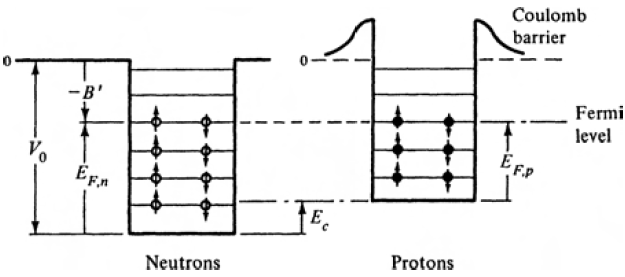
\includegraphics{fermi-gas-model}
                \caption{Esquema de los pozos de potencial en el modelo de Fermi.\parencite{das2003introduction}}
                \label{fig:FermiGasModel}
            \end{figure}
        \end{solution}
    \end{exercise}
\end{document}